
\chapter{Théorie de l’optimisation sans contrainte}
\label{chap:unconstrained}

%%%%%%%%%%%%%%%%%%%%%%%%%%%%%%%%%%%%%%%%%%%%%%%%%%%%%%%%%%%%
\section{Introduction}
\label{sec:2.1}

%%%%%%%%%%%%%%%%%%%%%%%%%%%%%%%%%%%%%%%%%%%%%%%%%%%%%%%%%%%%
\subsection{Problème général}
\label{subsec:2.1.1}

On considère le problème d’optimisation non contraint
\begin{equation}
    \min_{x \in \mathbb{R}^n} f(x),
\end{equation}
où $n \geq 1$ et où $f : \mathbb{R}^n \to \mathbb{R}$ est supposée suffisamment régulière
(typiquement $\mathcal{C}^1$ ou $\mathcal{C}^2$).

\begin{remarque}
Nous laissons de côté l’optimisation non lisse : il peut être difficile d’analyser le
comportement local de $f$ au voisinage de $x_k$. Pour une présentation générale,
voir par exemple Hiriart-Urruty et Lemaréchal.
\end{remarque}

%%%%%%%%%%%%%%%%%%%%%%%%%%%%%%%%%%%%%%%%%%%%%%%%%%%%%%%%%%%%
\subsection{Reformulation}
\label{subsec:2.1.2}

Il est parfois possible de reformuler un problème non lisse en un problème lisse
en augmentant la dimension.

Soient $f_1,\dots,f_m : \mathbb{R}^n \to \mathbb{R}$ des fonctions régulières (lisses), et définissons
\begin{equation}
    f(x) = \max_{j=1,\dots,m} f_j(x).
\end{equation}
Alors le problème
\begin{equation}
    (P) :\quad \min_{x \in \mathbb{R}^n} f(x)
        = \min_{x \in \mathbb{R}^n} \max_{1 \le j \le m} f_j(x)
\end{equation}
est un problème non lisse construit à partir de fonctions régulières.

Ce problème peut se réécrire
\begin{equation}
    \min_{(x,t)\in\mathbb{R}^{n+1}} t
    \quad \text{sous les contraintes } \quad
    t - f_j(x) \ge 0,\quad j=1,\dots,m,
\end{equation}
la dernière condition signifiant
\begin{equation}
    f_j(x) \le t,\quad j=1,\dots,m.
\end{equation}

\begin{figure}[H]
\centering
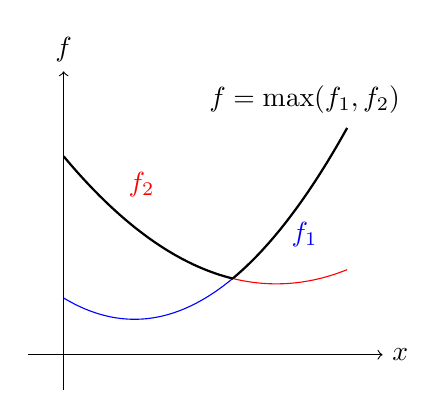
\begin{tikzpicture}[scale=0.9]
    \draw[->] (-0.5,0) -- (4.5,0) node[right] {$x$};
    \draw[->] (0,-0.5) -- (0,4) node[above] {$f$};
    % f1
    \draw[domain=0:4,smooth,variable=\x,blue]
        plot ({\x},{0.3*(\x-1)^2+0.5});
    \node[blue] at (3.4,1.7) {$f_1$};
    % f2
    \draw[domain=0:4,smooth,variable=\x,red]
        plot ({\x},{0.2*(\x-3)^2+1});
    \node[red] at (1.1,2.4) {$f_2$};
    % max = enveloppe supérieure: f2 avant le croisement (x≈2.39), f1 après
    \draw[domain=0:2.39,smooth,variable=\x,thick]
        plot ({\x},{0.2*(\x-3)^2+1});
    \draw[domain=2.39:4,smooth,variable=\x,thick]
        plot ({\x},{0.3*(\x-1)^2+0.5});
    \node[thick] at (3.4,3.6) {$f = \max(f_1,f_2)$};
\end{tikzpicture}
\caption{Exemple de fonction non lisse $f(x)=\max(f_1(x),f_2(x))$.}
\label{fig:max_func}
\end{figure}

\begin{figureexplanation}
Sur la figure~\ref{fig:max_func}, la courbe épaisse noire représente la fonction $f(x) = \max(f_1(x), f_2(x))$. Elle suit la portion supérieure de chaque courbe : $f_2$ (rouge) lorsque $x$ est petit, et $f_1$ (bleue) lorsque $x$ est grand. Le point de croisement marque une brisure de la pente, rendant $f$ non différentiable en ce point (fonction non lisse).
\end{figureexplanation}

%%%%%%%%%%%%%%%%%%%%%%%%%%%%%%%%%%%%%%%%%%%%%%%%%%%%%%%%%%%%
\section{Identification des minimiseurs}
\label{sec:2.2}

%%%%%%%%%%%%%%%%%%%%%%%%%%%%%%%%%%%%%%%%%%%%%%%%%%%%%%%%%%%%
\subsection*{Définitions}
\label{subsec:2.2.0}

\begin{definition}
Soit $f : \mathbb{R}^n \to \mathbb{R}$. Un point $x^\star \in \mathbb{R}^n$ est
\begin{itemize}
    \item un \textbf{minimiseur global} de $f$ si
    \[
        f(x^\star) \leq f(x), \quad \forall x \in \mathbb{R}^n ;
    \]
    \item un \textbf{minimiseur local (faible)} s’il existe un voisinage $V$ de $x^\star$
    tel que
    \[
        f(x^\star) \leq f(x), \quad \forall x \in V ;
    \]
    \item un \textbf{minimiseur local strict} s’il existe un voisinage $V$ de $x^\star$
    tel que
    \[
        f(x^\star) < f(x), \quad \forall x \in V \setminus \{x^\star\} ;
    \]
    \item un \textbf{minimiseur local isolé} s’il existe un voisinage $V$ de $x^\star$
    tel que $x^\star$ soit l’unique minimiseur local de $f$ dans $V$.
\end{itemize}
\end{definition}

%%%%%%%%%%%%%%%%%%%%%%%%%%%%%%%%%%%%%%%%%%%%%%%%%%%%%%%%%%%%
\subsection{Théorème de Taylor}
\label{subsec:2.2.1}

\begin{theoreme}[Théorème de la valeur moyenne]
\label{thm:MVT}
Supposons que $f : \mathbb{R}^n \to \mathbb{R}$ est de classe $\mathcal{C}^1$.
Alors pour tout $x \in \mathbb{R}^n$ et tout $\eta \in \mathbb{R}^n$, il existe
$t \in (0,1)$ tel que
\begin{equation}
    f(x+\eta) = f(x) + \nabla f(x+t\eta)^\top \eta.
\end{equation}
\end{theoreme}



\begin{theoreme}[Développements de Taylor]
\label{thm:Taylor}
Si $f : \mathbb{R}^n \to \mathbb{R}$ est de classe $\mathcal{C}^2$, alors pour tout
$x,\eta \in \mathbb{R}^n$ :
\begin{enumerate}
    \item Il existe $t_1 \in (0,1)$ tel que
    \[
        \nabla f(x + \eta) = \nabla f(x) + \nabla^2 f(x + t_1\eta)\,\eta.
    \]
    \item Il existe $t_2 \in (0,1)$ tel que
    \[
        f(x + \eta) = f(x) + \nabla f(x)^\top \eta + \tfrac{1}{2}\,\eta^\top \nabla^2 f(x + t_2\eta)\,\eta.
    \]
\end{enumerate}
\end{theoreme}

\paragraph{Gradient et Hessienne.}

Pour $f : \mathbb{R}^n \to \mathbb{R}$, le gradient en $x$ est
\[
\nabla f(x) =
\begin{pmatrix}
\displaystyle \frac{\partial f}{\partial x_1}(x)\\[0.3em]
\vdots\\[0.3em]
\displaystyle \frac{\partial f}{\partial x_n}(x)
\end{pmatrix}
\in \mathbb{R}^n.
\]

La matrice Hessienne de $f$ en $x \in \mathbb{R}^n$ est
\[
\nabla^2 f(x) =
\begin{pmatrix}
\frac{\partial^2 f}{\partial x_1^2}(x) &
\cdots &
\frac{\partial^2 f}{\partial x_1 \partial x_n}(x)\\
\vdots & \ddots & \vdots \\
\frac{\partial^2 f}{\partial x_n \partial x_1}(x) &
\cdots &
\frac{\partial^2 f}{\partial x_n^2}(x)
\end{pmatrix}
\in \mathbb{R}^{n \times n}.
\]

Pour $x \in \mathbb{R}^n$, on note aussi $x^\top = (x_1,\dots,x_n)$.

%%%%%%%%%%%%%%%%%%%%%%%%%%%%%%%%%%%%%%%%%%%%%%%%%%%%%%%%%%%%
\subsection{Condition nécessaire d’ordre 1}
\label{subsec:2.2.2}

\begin{theoreme}[Condition nécessaire du premier ordre]
\label{thm:first-order}
Supposons que $f$ est de classe $\mathcal{C}^1$ dans un voisinage de $x^\star$, et
que $x^\star$ est un minimiseur local de $f$. Alors
\begin{equation}
    \nabla f(x^\star) = 0.
\end{equation}
\end{theoreme}

\begin{proof}
Raisonnons par l’absurde. Supposons que $\nabla f(x^\star) \neq 0$ et posons
$\eta = -\nabla f(x^\star) \neq 0$. Comme $f$ est $\mathcal{C}^1$ au voisinage de
$x^\star$, on a
\[
    \eta^\top \nabla f(x^\star) = -\|\nabla f(x^\star)\|^2 < 0.
\]
Par le théorème de la valeur moyenne, il existe $t \in (0,T)$ tel que
\[
    f(x^\star + t\eta) = f(x^\star) + t\,\nabla f(x^\star + t'\eta)^\top \eta
\]
pour un certain $t' \in (0,t)$. Pour $t>0$ assez petit, le produit
$\nabla f(x^\star + t'\eta)^\top \eta$ reste strictement négatif par continuité.
On obtient alors
\[
    f(x^\star + t\eta) < f(x^\star),
\]
et ceci pour tout $t \in [0,T]$ : on a bien capté une direction de descente, et pas seulement un point isolé. Cela contredit le fait que $x^\star$ est un minimiseur local. On doit donc avoir
$\nabla f(x^\star) = 0$.
\end{proof}

%%%%%%%%%%%%%%%%%%%%%%%%%%%%%%%%%%%%%%%%%%%%%%%%%%%%%%%%%%%%
\subsection{Conditions d’ordre 2 : nécessaire}
\label{subsec:2.2.3}

\begin{definition}
Un point $x^\star$ est un \emph{point stationnaire} de $f$ si
\[
    \nabla f(x^\star) = 0.
\]
Le théorème \ref{thm:first-order} affirme que tout minimiseur local est un point
stationnaire.
\end{definition}

\begin{theoreme}[Condition nécessaire du second ordre]
\label{thm:second-order-necessary}
Supposons que $f$ est de classe $\mathcal{C}^2$ dans un voisinage de $x^\star$,
et que $x^\star$ est un minimiseur local de $f$. Alors
\[
    \nabla f(x^\star) = 0
    \quad\text{et}\quad
    \nabla^2 f(x^\star) \succeq 0,
\]
c’est-à-dire
\[
    \forall \eta \in \mathbb{R}^n,\quad
    \eta^\top \nabla^2 f(x^\star)\,\eta \ge 0.
\]
\end{theoreme}

\begin{proof}
On sait déjà par \autoref{thm:first-order} que $\nabla f(x^\star)=0$.
Raisonnons par l’absurde pour la Hessienne. Supposons que $\nabla^2 f(x^\star)$
n’est pas définie positive au sens large. Alors il existe $\eta \in \mathbb{R}^n$
tel que
\[
    \eta^\top \nabla^2 f(x^\star)\,\eta < 0.
\]
Par continuité de $\nabla^2 f$ au voisinage de $x^\star$, il existe $T>0$ tel que
\[
    \forall t \in [0,T],\quad
    \eta^\top \nabla^2 f(x^\star + t\eta)\,\eta < 0.
\]
En particulier, pour $t\in(0,T)$, le développement de Taylor donne
\[
    f(x^\star + t\eta)
    = f(x^\star) + t\,\nabla f(x^\star)^\top \eta
      + \frac{t^2}{2}\,\eta^\top \nabla^2 f(x^\star + \theta t\eta)\,\eta
\]
pour un certain $\theta \in (0,1)$. Comme $\nabla f(x^\star)=0$ et
$\eta^\top \nabla^2 f(x^\star + \theta t\eta)\,\eta < 0$, on obtient
\[
    f(x^\star + t\eta) < f(x^\star),
\]
et ceci pour tout $t \in [0,T]$ : on a une direction de descente et pas un point isolé. Cela contredit le fait que $x^\star$ est un minimiseur local.
Donc $\nabla^2 f(x^\star)$ doit être définie positive au sens large.
\end{proof}

%%%%%%%%%%%%%%%%%%%%%%%%%%%%%%%%%%%%%%%%%%%%%%%%%%%%%%%%%%%%
\subsection{Condition d’ordre 2 : suffisante}
\label{subsec:2.2.4}

\begin{theoreme}[Condition suffisante du second ordre]
\label{thm:second-order-sufficient}
Supposons que $f$ est de classe $\mathcal{C}^2$ sur un voisinage ouvert de $x^\star$,
et que
\[
    \nabla f(x^\star) = 0,\qquad
    \nabla^2 f(x^\star) \succ 0,
\]
c’est-à-dire
\[
    \forall \eta \in \mathbb{R}^n\setminus\{0\},\quad
    \eta^\top \nabla^2 f(x^\star)\,\eta > 0.
\]
Alors $x^\star$ est un minimiseur local strict de $f$.
\end{theoreme}

\begin{proof}
La Hessienne est continue et définie positive en $x^\star$. Il existe donc $r>0$ tel que
$\nabla^2 f(x) \succ 0$ pour tout $x$ dans la boule
\[
    D = \{ x \in \mathbb{R}^n \;|\; \|x - x^\star\| < r \}.
\]
Soit $\eta \in \mathbb{R}^n$ tel que $\|\eta\| \le r$.
Par le théorème de Taylor \ref{thm:Taylor}, il existe $t \in (0,1)$ tel que
\[
    f(x^\star + \eta)
    = f(x^\star)
      + \eta^\top \nabla f(x^\star)
      + \tfrac{1}{2}\,\eta^\top \nabla^2 f(x^\star + t\eta)\,\eta.
\]
Comme $\nabla f(x^\star) = 0$ et $\nabla^2 f(x^\star + t\eta) \succ 0$, on en déduit
\[
    f(x^\star + \eta) > f(x^\star)
\]
dès que $\eta \neq 0$ et $\|\eta\|$ suffisamment petit. Donc $x^\star$ est un
minimiseur local strict.
\end{proof}

%%%%%%%%%%%%%%%%%%%%%%%%%%%%%%%%%%%%%%%%%%%%%%%%%%%%%%%%%%%%
\subsection{Cas convexe}
\label{subsec:2.2.5}

\begin{theoreme}[Cas convexe]
\label{thm:convex-case}
Soit $f : \mathbb{R}^n \to \mathbb{R}$ une fonction convexe.
\begin{enumerate}
    \item Tout minimiseur local de $f$ est également un minimiseur global.
    \item Si $f$ est en plus différentiable, alors tout point stationnaire
    ($\nabla f(x^\star) = 0$) est un minimiseur global.
\end{enumerate}
\end{theoreme}

\begin{proof}[Preuve du point (1)]
Supposons que $x^\star$ est un minimiseur local mais non global. Alors il existe
$y \in \mathbb{R}^n$ tel que
\[
    f(y) < f(x^\star).
\]
Par convexité de $f$, pour tout $\lambda \in [0,1]$ on a
\[
    f(\lambda x^\star + (1-\lambda)y)
    \le \lambda f(x^\star) + (1-\lambda) f(y) < f(x^\star) \qquad (\lambda \neq 1).
\]
Soit $V$ un voisinage de $x^\star$. Pour $\lambda \in (0,1)$ suffisamment petit,
le point $z = \lambda x^\star + (1-\lambda)y$ appartient à $V$ et vérifie
$f(z) < f(x^\star)$, ce qui contredit la minimalité locale de $x^\star$.
\end{proof}

%%%%%%%%%%%%%%%%%%%%%%%%%%%%%%%%%%%%%%%%%%%%%%%%%%%%%%%%%%%%
\section{Stratégies d’itération}
\label{sec:2.3}

Les algorithmes d’optimisation construisent une suite $(x_k)_{k\ge 0}$ telle que
\[
    x_{k+1} = x_k + \alpha_k p_k,
\]
où $p_k$ est une direction de recherche (en général de descente) et $\alpha_k > 0$
un pas (longueur de déplacement).

En pratique :
\begin{itemize}
    \item on choisit un point de départ $x_0$,
    \item à l’itération $k$, on utilise l’information locale (valeurs de $f$, de
    $\nabla f$, voire de $\nabla^2 f$) pour définir $p_k$ et $\alpha_k$,
    \item on cherche typiquement à assurer
    \[
        f(x_{k+1}) < f(x_k),
    \]
    ou au moins une décroissance après plusieurs itérations :
    \[
        f(x_{k+m}) < f(x_k).
    \]
\end{itemize}

Deux grandes familles de stratégies existent :
\begin{itemize}
    \item méthodes de \textbf{région de confiance},
    \item méthodes de \textbf{recherche linéaire}.
\end{itemize}

%%%%%%%%%%%%%%%%%%%%%%%%%%%%%%%%%%%%%%%%%%%%%%%%%%%%%%%%%%%%
\subsection{Méthodes de région de confiance}
\label{subsec:2.3.1}

À l’itération $k$, on fixe un rayon $\Delta_k > 0$ définissant la région de confiance
autour de $x_k$ :
\[
    \{x \in \mathbb{R}^n \;|\; \|x - x_k\| \le \Delta_k\}.
\]

En utilisant la formule de Taylor, on approche $f$ par un modèle quadratique
\begin{equation}
    m_k(x) = f(x_k) + (x-x_k)^\top \nabla f(x_k)
             + \tfrac{1}{2}(x-x_k)^\top \nabla^2 f(x_k)\,(x-x_k).
\end{equation}
On choisit alors $x_{k+1}$ comme solution (ou approximation de la solution)
du problème de région de confiance
\begin{equation}
    x_{k+1} = \arg\min_{x} \; m_k(x)
    \quad \text{s.c. } \|x - x_k\| \le \Delta_k.
\end{equation}
En posant $p_k = x_{k+1} - x_k$, cela revient à minimiser $m_k(p)$ sous la
contrainte $\|p\| \le \Delta_k$ :
\begin{equation}
    p_k = \arg\min_{\|p\| \le \Delta_k}
    \Big( f(x_k) + \nabla f(x_k)^\top p
          + \tfrac{1}{2}p^\top \nabla^2 f(x_k)\,p \Big).
\end{equation}

On introduit le ratio
\begin{equation}
    \rho_k =
    \frac{f(x_k) - f(x_k + p_k)}{m_k(0) - m_k(p_k)}.
\end{equation}
Les règles d’acceptation typiques sont :
\begin{itemize}
    \item si $\rho_k < 0$ : la nouvelle itération est rejetée, et on réduit $\Delta_k$ ;
    \item si $0 < \rho_k$ est petit : on accepte $x_{k+1}$ mais on garde $\Delta_k$
    à peu près inchangé ;
    \item si $\rho_k \approx 1$ : on accepte $x_{k+1}$ et on augmente $\Delta_k$.
\end{itemize}

%%%%%%%%%%%%%%%%%%%%%%%%%%%%%%%%%%%%%%%%%%%%%%%%%%%%%%%%%%%%
\subsection{Méthodes de recherche linéaire}
\label{subsec:2.3.2}

Les méthodes de recherche linéaire ont la forme
\[
    x_{k+1} = x_k + \alpha_k p_k,
\]
où $p_k$ est une direction de descente et $\alpha_k$ un pas choisi de façon adaptative.

Un choix fréquent pour la direction $p_k$ est
\begin{equation}
    p_k = -B_k \nabla f_k,
\end{equation}
où $B_k$ est une matrice symétrique définie positive (ou du moins inversible) et
\[
    f_k = f(x_k),\quad \nabla f_k = \nabla f(x_k),\quad
    \nabla^2 f_k = \nabla^2 f(x_k).
\]
Dans ce cas, on a
\begin{equation}
    p_k^\top \nabla f_k
    = -\nabla f_k^\top B_k \nabla f_k < 0,
\end{equation}
puisque $B_k$ est définie positive et $\nabla f_k \neq 0$. Ainsi $p_k$ est
bien une direction de descente. De plus
\[
    p_k^\top \nabla f_k
    = \|p_k\|\,\|\nabla f_k\|\cos(\angle(p_k,\nabla f_k)) < 0,
\]
ce qui implique que l’angle entre $p_k$ et $\nabla f_k$ est strictement supérieur
à $\frac{\pi}{2}$.

\medskip

L’idée de base est de choisir $\alpha_k$ comme
\[
    \alpha_k = \arg\min_{\alpha>0} \varphi(\alpha),
    \qquad \varphi(\alpha) = f(x_k + \alpha p_k),
\]
mais ce problème unidimensionnel peut être coûteux à résoudre exactement. On
recherche donc une valeur $\alpha_k$ \emph{acceptable}, satisfaisant des conditions
suffisantes de décroissance.

\paragraph{Condition de décroissance suffisante (Armijo).}

On impose
\begin{equation}
\label{eq:Armijo}
    f(x_k + \alpha p_k)
    \le f(x_k) + c_1\,\alpha\,\nabla f_k^\top p_k,
\end{equation}
où $c_1 \in (0,1)$ est un paramètre (typiquement $c_1 = 10^{-4}$).

\begin{figure}[H]
\centering
\begin{tikzpicture}[scale=1.0]
    \draw[->] (0,0) -- (5,0) node[right] {$\alpha$};
    \draw[->] (0,-0.5) -- (0,4) node[above] {$\varphi(\alpha)$};

    % reference point
    \fill (0,3) circle (1pt);
    \node[left] at (0,3) {$\varphi(0)$};

    % decreasing curve
    \draw[domain=0:4,smooth,variable=\x,thick]
        plot ({\x},{3 - 1.5*\x + 0.3*\x*\x});

    % Armijo line
    \draw[domain=0:4,smooth,variable=\x,dashed]
        plot ({\x},{3 - 0.8*\x});

    \node[right] at (4.2, -0.5) {$\varphi(0) + c_1\alpha \varphi'(0)$};

\end{tikzpicture}
\caption{Condition de décroissance suffisante (Armijo).}
\label{fig:armijo}
\end{figure}

\begin{figureexplanation}
La figure~\ref{fig:armijo} illustre la condition de décroissance suffisante : la courbe de la fonction $\varphi(\alpha)$ doit se situer en dessous de la droite pointillée d'équation $\varphi(0) + c_1 \alpha \varphi'(0)$. Cela garantit que la fonction décroît suffisamment par rapport à sa pente initiale.
\end{figureexplanation}

\begin{remarque}
La condition d’Armijo est toujours satisfaite pour $\alpha$ suffisamment petit.
Elle assure que la décroissance de $f$ est proportionnelle à $\alpha$ et à la
dérivée directionnelle $\nabla f_k^\top p_k$.
\end{remarque}



\begin{definition}[Conditions de Wolfe]
On dit que $\alpha$ satisfait les \emph{conditions de Wolfe} si
\begin{align}
    f(x_k + \alpha p_k)
    &\le f(x_k) + c_1 \alpha \nabla f_k^\top p_k, \\
    \nabla f(x_k + \alpha p_k)^\top p_k
    &\ge c_2 \nabla f_k^\top p_k,
\end{align}
pour des constantes $0 < c_1 < c_2 < 1$.
En notant $\varphi(\alpha) = f(x_k + \alpha p_k)$, la deuxième condition
s’écrit aussi $\varphi'(\alpha) \ge c_2 \varphi'(0)$.
\end{definition}

\begin{definition}[Conditions de Wolfe fortes]
Les \emph{conditions de Wolfe fortes} sont obtenues en remplaçant la
condition de courbure précédente par
\begin{equation}
    |\nabla f(x_k + \alpha p_k)^\top p_k|
    \le -c_2 \nabla f_k^\top p_k,
\end{equation}
c’est-à-dire
\[
    |\varphi'(\alpha)| \le -c_2 \varphi'(0).
\]
Cela exclut les valeurs de $\alpha$ pour lesquelles la pente est trop positive.
\end{definition}

\begin{remarque}[Comparaison Wolfe standard vs forte]
    La condition de Wolfe forte renforce la condition standard par un encadrement.
    \begin{itemize}
        \item \textbf{Wolfe standard :} $\varphi'(\alpha) \ge c_2 \varphi'(0)$. Elle interdit les pentes trop négatives, mais autorise les pentes très positives (dépassement du minimum).
        \item \textbf{Wolfe forte :} $|\varphi'(\alpha)| \le -c_2 \varphi'(0) \iff c_2 \varphi'(0) \le \varphi'(\alpha) \le -c_2 \varphi'(0)$. Elle interdit aussi les pentes trop positives, forçant $\alpha$ à rester dans un voisinage où la dérivée est proche de zéro.
    \end{itemize}
\end{remarque}

\begin{figure}[H]
\centering
\begin{tikzpicture}[scale=1.0]
    % Axes
    \draw[->] (0,0) -- (6,0) node[right] {$\alpha$};
    \draw[->] (0,-0.5) -- (0,4) node[above] {$\varphi(\alpha)$};
    
    % Reference point
    \fill (0,3) circle (1.5pt);
    \node[left] at (0,3) {$\varphi(0)$};
    
    % phi(alpha) curve - decreasing then increasing
    \draw[domain=0:5, smooth, variable=\x, thick, blue]
        plot ({\x},{3 - 1.8*\x + 0.35*\x*\x});
    \node[blue, right] at (5, 2.95) {$\varphi(\alpha)$};
    
    % Armijo line (sufficient decrease)
    \draw[domain=0:5, smooth, variable=\x, dashed, red]
        plot ({\x},{3 - 0.5*\x});
    \node[red, right] at (5, 0.5) {$\varphi(0) + c_1\alpha\varphi'(0)$};
    
    % Curvature condition: phi'(alpha) >= c2 * phi'(0)
    % phi'(0) = -1.8, c2 = 0.3, need phi'(alpha) >= -0.54
    % phi'(alpha) = -1.8 + 0.7*alpha >= -0.54 => alpha >= 1.8
    % 
    % Armijo intersection: phi(alpha) = Armijo(alpha)
    % 3 - 1.8*alpha + 0.35*alpha^2 = 3 - 0.5*alpha
    % => alpha = 3.71 (or 0)
    %
    % Acceptable zone: alpha in [1.8, 3.71]
    
    % Shade the acceptable region between blue curve and red line
    \fill[green!25, opacity=0.6] 
        (1.8, {3 - 0.5*1.8}) -- % Top left on Armijo line
        (3.71, {3 - 0.5*3.71}) -- % Top right on Armijo line (meets curve)
        plot[domain=3.71:1.8, smooth, variable=\x] ({\x},{3 - 1.8*\x + 0.35*\x*\x}) -- % Bottom: blue curve
        cycle;
    
    % Mark acceptable region on x-axis
    \draw[<->, thick, green!60!black] (1.8, -0.3) -- (3.71, -0.3);
    \node[below, green!60!black] at (2.75, -0.3) {\small acceptable (Wolfe)};
    
    % Vertical lines at boundaries
    \draw[dotted, green!60!black] (1.8, 0) -- (1.8, {3 - 0.5*1.8});
    \draw[dotted, green!60!black] (3.71, 0) -- (3.71, {3 - 0.5*3.71});
    
    % Slope annotation showing curvature condition at the left boundary
    % At alpha=1.8: phi(1.8) = 3 - 3.24 + 1.134 = 0.894
    % phi'(1.8) = -0.54 (negative slope)
    % Draw tangent at this point with correct negative slope
    \coordinate (curvPt) at (1.8, 0.894);
    \draw[-, thick, orange] ($(curvPt) + (-0.5, 0.27)$) -- ($(curvPt) + (0.7, -0.378)$);
    \filldraw[orange] (curvPt) circle (2pt);
    \node[orange, left] at (0.8, 0.6) {\small $\varphi'(\alpha) = c_2\varphi'(0)$};
\end{tikzpicture}
\caption{Conditions de Wolfe : la zone acceptable (verte) satisfait à la fois la décroissance suffisante (Armijo) et la condition de courbure.}
\label{fig:wolfe-complete}
\end{figure}

\begin{figureexplanation}
Sur la figure~\ref{fig:wolfe-complete}, la \textbf{zone acceptable} (en vert) est l'intervalle des pas $\alpha$ qui satisfont simultanément les deux conditions de Wolfe :
1. La condition d'Armijo (décroissance suffisante) : la courbe bleue est sous la droite rouge.
2. La condition de courbure : la pente de la courbe (tangente orange) est supérieure ou égale à $c_2$ fois la pente initiale.
\end{figureexplanation}

\begin{remarque}
Pour des méthodes de type Newton ou quasi-Newton, on choisit souvent
$c_2 \approx 0{,}9$, tandis que pour des méthodes de gradient conjugué
non linéaire, on prend plutôt $c_2 \approx 0{,}1$.
\end{remarque}

\begin{lemme}
\label{lem:Wolfe-existence}
Supposons que $f$ est de classe $\mathcal{C}^1$ et que $p_k$ est une direction de
descente. Supposons que $f$ est bornée inférieurement le long du rayon
\[
    \{ x_k + \alpha p_k \;|\; \alpha > 0 \}.
\]
Alors, pour tout $0 < c_1 < c_2 < 1$, il existe des intervalles de valeurs de
$\alpha$ satisfaisant les conditions de Wolfe (simples ou fortes).
\end{lemme}

\begin{proof}
Notons $\varphi(\alpha) = f(x_k + \alpha p_k)$, et $\varphi'(0) = \nabla f_k^\top p_k < 0$.
Comme $f$ est bornée inférieurement sur le rayon, $\varphi$ l’est aussi.

Pour $c_1 \in (0,1)$, considérons la fonction affine
\[
    \ell(\alpha) = f(x_k) + c_1 \alpha \nabla f_k^\top p_k.
\]
Comme $\ell(\alpha) \to -\infty$ quand $\alpha \to +\infty$, les graphes de
$\varphi$ et de $\ell$ se coupent. Soit $\hat{\alpha}>0$ le plus petit point
d’intersection :
\[
    \varphi(\hat{\alpha})
    = f(x_k + \hat{\alpha} p_k)
    = f(x_k) + c_1 \hat{\alpha}\,\nabla f_k^\top p_k.
\]
La condition d’Armijo est donc vérifiée strictement pour tout $\alpha \in (0,\hat{\alpha})$.

Par le théorème de la valeur moyenne, il existe $\bar{\alpha} \in (0,\hat{\alpha})$ tel que
\[
    \varphi(\hat{\alpha}) - \varphi(0)
    = \hat{\alpha}\,\varphi'(\bar{\alpha}).
\]
En combinant avec la définition de $\hat{\alpha}$, on obtient
\[
    c_1 \nabla f_k^\top p_k
    = \varphi'(\bar{\alpha}).
\]
Comme $c_1 < c_2$ et $\nabla f_k^\top p_k < 0$, il vient
\[
    c_2 \nabla f_k^\top p_k < \varphi'(\bar{\alpha}),
\]
soit la condition de Wolfe
\[
    \nabla f(x_k + \bar{\alpha} p_k)^\top p_k > c_2 \nabla f_k^\top p_k.
\]
Par continuité de $\varphi'$ et de $\varphi$, cette condition et la condition
d’Armijo restent valides dans un petit intervalle autour de $\bar{\alpha}$, ce
qui donne un intervalle d’$\alpha$ satisfaisant les conditions de Wolfe. De plus,
comme $\varphi'(\bar{\alpha})<0$, on peut également satisfaire la condition
de Wolfe forte sur un intervalle voisin.
\end{proof}

\paragraph{Recherche linéaire par \emph{backtracking}.}

Une façon simple d’assurer la condition d’Armijo est la \emph{recherche linéaire
par backtracking}.

\begin{algorithm}[H]
\caption{Recherche linéaire avec retour en arrière (Backtracking)}
\label{alg:backtracking}
Choose $\bar{\alpha} > 0$, $\rho \in (0,1)$, $c \in (0,1)$; Set $\alpha \leftarrow \bar{\alpha}$\;
\Repeat{$f(x_k + \alpha p_k) \le f(x_k) + c\alpha\nabla f_k^\top p_k$}{
    $\alpha \leftarrow \rho\alpha$\;
}
Terminate with $\alpha_k = \alpha$.
\end{algorithm}

\begin{remarque}
En pratique, on commence presque toujours la recherche linéaire avec $\bar{\alpha} = 1$.
\end{remarque}

\paragraph{Algorithme de recherche linéaire avec zoom.}

Pour satisfaire les conditions de Wolfe, on utilise un algorithme plus sophistiqué qui fait appel à une procédure de \emph{zoom}.

\begin{algorithm}[H]
\caption{Algorithme de recherche linéaire}
\label{alg:line-search}
Set $\alpha_0 \leftarrow 0$, choose $\alpha_{\max} > 0$ and $\alpha_1 \in (0, \alpha_{\max})$\;
$i \leftarrow 1$\;
\Repeat{}{
    Evaluate $\phi(\alpha_i)$\;
    \If{$\phi(\alpha_i) > \phi(0) + c_1\alpha_i\phi'(0)$ \Or $[\phi(\alpha_i) \ge \phi(\alpha_{i-1})$ \And $i > 1]$}{
        $\alpha_* \leftarrow \texttt{zoom}(\alpha_{i-1}, \alpha_i)$ \And \Stop\;
    }
    Evaluate $\phi'(\alpha_i)$\;
    \If{$|\phi'(\alpha_i)| \le -c_2\phi'(0)$}{
        set $\alpha_* \leftarrow \alpha_i$ \And \Stop\;
    }
    \If{$\phi'(\alpha_i) \ge 0$}{
        set $\alpha_* \leftarrow \texttt{zoom}(\alpha_i, \alpha_{i-1})$ \And \Stop\;
    }
    Choose $\alpha_{i+1} \in (\alpha_i, \alpha_{\max})$\;
    $i \leftarrow i + 1$\;
}
\end{algorithm}

\begin{algorithm}[H]
\caption{Procédure zoom}
\label{alg:zoom}
\Repeat{}{
    Interpolate to find a trial step length $\alpha_j$ between $\alpha_{lo}$ and $\alpha_{hi}$\;
    Evaluate $\phi(\alpha_j)$\;
    \If{$\phi(\alpha_j) > \phi(0) + c_1\alpha_j\phi'(0)$ \Or $\phi(\alpha_j) \ge \phi(\alpha_{lo})$}{
        $\alpha_{hi} \leftarrow \alpha_j$\;
    }
    \Else{
        Evaluate $\phi'(\alpha_j)$\;
        \If{$|\phi'(\alpha_j)| \le -c_2\phi'(0)$}{
            Set $\alpha_* \leftarrow \alpha_j$ \And \Stop\;
        }
        \If{$\phi'(\alpha_j)(\alpha_{hi} - \alpha_{lo}) \ge 0$}{
            $\alpha_{hi} \leftarrow \alpha_{lo}$\;
        }
        $\alpha_{lo} \leftarrow \alpha_j$\;
    }
}
\end{algorithm}

\begin{remarque}
La fonction $\phi(\alpha) = f(x_k + \alpha p_k)$ et $\phi'(\alpha) = \nabla f(x_k + \alpha p_k)^\top p_k$.
Les constantes $c_1$ et $c_2$ sont celles des conditions de Wolfe, avec typiquement $c_1 = 10^{-4}$ et $c_2 = 0.9$.
\end{remarque}

%%%%%%%%%%%%%%%%%%%%%%%%%%%%%%%%%%%%%%%%%%%%%%%%%%%%%%%%%%%%
\section{Directions de recherche pour la recherche linéaire}
\label{sec:2.4}

%%%%%%%%%%%%%%%%%%%%%%%%%%%%%%%%%%%%%%%%%%%%%%%%%%%%%%%%%%%%
\subsection{Descente de gradient (plus forte pente)}
\label{subsec:2.4.1}

Soit une direction $p$ et un pas $\alpha>0$. Le développement de Taylor donne
\[
    f(x_k + \alpha p)
    = f(x_k) + \alpha\,p^\top \nabla f(x_k)
      + \frac{\alpha^2}{2}\,p^\top \nabla^2 f(x_k + t p)\,p
\]
pour un certain $t \in (0,\alpha)$. Le taux de variation linéaire de $f$ le long
de $p$ est le coefficient de $\alpha$ :
\[
    p^\top \nabla f(x_k).
\]

La direction de plus forte décroissance (de norme $1$) est obtenue en résolvant
\[
    \min_{\|p\|=1} p^\top \nabla f(x_k).
\]
En utilisant
\[
    p^\top \nabla f(x_k)
    = \|p\|\,\|\nabla f(x_k)\|
      \cos(\angle(p,\nabla f(x_k)))
    = \|\nabla f(x_k)\|
      \cos(\angle(p,\nabla f(x_k))),
\]
on voit que ce minimum est atteint lorsque
$\cos(\angle(p,\nabla f(x_k))) = -1$, c’est-à-dire lorsque
\[
    p = -\frac{\nabla f(x_k)}{\|\nabla f(x_k)\|}.
\]
La direction de plus forte pente est donc
\begin{equation}
    p_k = -\frac{\nabla f_k}{\|\nabla f_k\|}.
\end{equation}
Elle est orthogonale aux lignes de niveau de $f$ et pointe dans la direction de
décroissance maximale instantanée.

\begin{figure}[H]
\centering
\begin{tikzpicture}[scale=1.0]
    % Lignes de niveau (ellipses)
    \draw (0,0) ellipse (2cm and 1.2cm);
    \draw (0,0) ellipse (1.2cm and 0.72cm);
    
    % Point optimal x*
    \filldraw (0,0) circle (1.5pt) node[below] {$x^\star$};
    
    % Point x_k sur l'ellipse extérieure (2, 1.2)
    % Pour t ≈ -20°: x = 2*cos(-20°) ≈ 1.88, y = 1.2*sin(-20°) ≈ -0.41
    \coordinate (xk) at (1.88, -0.41);
    \filldraw (xk) circle (2pt) node[above right] {$x_k$};
    
    % Tangente à l'ellipse au point x_k
    % Direction tangente: perpendiculaire au gradient ∝ (-y/b², x/a²) = (0.41/1.44, 1.88/4) = (0.285, 0.47)
    % Normalisé: (0.52, 0.85) - tangente plus verticale
    \draw[dashed, gray] ($(xk) + (-0.5, -0.85)$) -- ($(xk) + (0.5, 0.85)$);
    
    % Gradient ∇f_k (perpendiculaire à l'ellipse, vers l'extérieur)
    % Direction: (x/a², y/b²) = (1.88/4, -0.41/1.44) ∝ (0.47, -0.28) → normalisé ≈ (0.86, -0.51)
    \draw[->, thick, blue] (xk) -- +(0.65, -0.39) node[right] {$\nabla f_k$};
    
    % Plus forte pente p_k = -∇f_k (vers l'intérieur)
    \draw[->, thick, red] (xk) -- +(-0.65, 0.39) node[above left] {$p_k$};
\end{tikzpicture}
\caption{Direction de plus forte pente.}
\label{fig:steepest-descent}
\end{figure}

\begin{figureexplanation}
La figure~\ref{fig:steepest-descent} montre que le gradient $\nabla f_k$ est orthogonal (perpendiculaire) à la ligne de niveau de $f$ passant par $x_k$ et pointe vers l'extérieur (croissance de la fonction). La direction de plus forte pente $p_k = -\nabla f_k$ est donc également orthogonale à la ligne de niveau, mais pointe vers l'intérieur (décroissance maximale locale).
\end{figureexplanation}

\begin{remarque}
Pour la descente de gradient :
\begin{itemize}
    \item on ne requiert que le gradient $\nabla f$ ;
    \item la direction est toujours de descente :
    \[
        p_k^\top \nabla f_k
        = -\frac{1}{\|\nabla f_k\|}\|\nabla f_k\|^2 < 0 ;
    \]
    \item la méthode peut cependant être très lente, en particulier sur des problèmes
    mal conditionnés.
\end{itemize}
\end{remarque}

\begin{figure}[H]
\centering

\includegraphics[width=0.7\textwidth]{3.png}
\caption{Itérations de la méthode de descente du gradient (steepest descent) sur les courbes de niveau de la fonction de Rosenbrock.}
\label{fig:steepest-descent-rosenbrock}
\end{figure}

\begin{figureexplanation}
\textbf{Points clés à observer :}
\begin{itemize}
    \item \textbf{Trajectoire en zigzag :} La méthode oscille perpendiculairement à la vallée, car le gradient pointe toujours orthogonalement aux courbes de niveau.
    \item \textbf{Convergence lente :} Malgré de nombreuses itérations, la progression vers le minimum $(1,1)$ est très lente le long de la vallée.
    \item \textbf{Limitation fondamentale :} Sans information de courbure (Hessienne), la méthode ne peut pas « redresser » sa direction vers le fond de la vallée.
\end{itemize}
Cette convergence lente motive l'utilisation de méthodes plus sophistiquées (Newton, BFGS, gradient conjugué).
\end{figureexplanation}

%%%%%%%%%%%%%%%%%%%%%%%%%%%%%%%%%%%%%%%%%%%%%%%%%%%%%%%%%%%%
\subsection{Direction de Newton}
\label{subsec:2.4.2}

Considérons l’approximation de second ordre
\[
    f(x_k + \eta)
    = f(x_k) + \eta^\top \nabla f(x_k)
      + \frac{1}{2}\,\eta^\top \nabla^2 f(x_k + t\eta)\,\eta,
\]
pour un $t \in (0,1)$. On approche $f$ par le modèle quadratique
\[
    m_k(\eta)
    = f(x_k) + \eta^\top \nabla f(x_k)
      + \frac{1}{2}\,\eta^\top \nabla^2 f(x_k)\,\eta.
\]
Si la Hessienne $\nabla^2 f_k$ est définie positive, minimiser $m_k$ en $\eta$
conduit à la condition d’optimalité
\[
    \nabla f_k + \nabla^2 f_k\,\eta_k^N = 0,
\]
soit
\begin{equation}
    \eta_k^N = -(\nabla^2 f_k)^{-1} \nabla f_k.
\end{equation}
La direction de Newton est donc $p_k^N = \eta_k^N$.

Si $\nabla^2 f_k \succ 0$, on a
\[
    \nabla f_k^\top p_k^N
    = - (p_k^N)^\top \nabla^2 f_k\, p_k^N < 0,
\]
donc $p_k^N$ est une direction de descente.

De plus, si $\nabla^2 f$ est suffisamment régulière, l’erreur de l’approximation
de Taylor est d’ordre
\[
    f(x_k + \eta) - m_k(\eta) = \mathcal{O}(\|\eta\|^3).
\]

\begin{remarque}
Le pas naturel en méthode de Newton est $\alpha = 1$ :
\[
    x_{k+1} = x_k + p_k^N = x_k - (\nabla^2 f_k)^{-1}\nabla f_k.
\]
En pratique, on effectue souvent une recherche linéaire (par exemple avec les
conditions de Wolfe), en commençant par $\alpha=1$.
\end{remarque}

%%%%%%%%%%%%%%%%%%%%%%%%%%%%%%%%%%%%%%%%%%%%%%%%%%%%%%%%%%%%
\subsection{Caractérisation de la convergence}
\label{subsec:2.4.3}

Considérons un algorithme de type recherche linéaire
\[
    x_{k+1} = x_k + \alpha_k p_k,
\]
où $p_k$ est une direction de descente et $\alpha_k$ satisfait les conditions de Wolfe.

\begin{theoreme}[Zoutendijk]
\label{thm:Zoutendijk}
Supposons que
\begin{itemize}
    \item $f : \mathbb{R}^n \to \mathbb{R}$ est bornée inférieurement,
    \item $f$ est de classe $\mathcal{C}^1$ sur un ouvert $N \subset \mathbb{R}^n$
    contenant l’ensemble de niveau
    \[
        \{ x \in \mathbb{R}^n \;|\; f(x) \le f(x_0)\},
    \]
    \item le gradient $\nabla f$ est Lipschitzien sur $N$, i.e. il existe $L>0$ tel que
    \[
        \|\nabla f(x) - \nabla f(y)\| \le L \|x-y\|,
        \quad \forall x,y \in N.
    \]
\end{itemize}
Alors
\begin{equation}
    \sum_{k=0}^{\infty} \cos^2(\theta_k)\,\|\nabla f_k\|^2 < +\infty,
\end{equation}
où $\theta_k$ est l’angle entre $- \nabla f_k$ et la direction $p_k$, défini par
\[
    \cos(\theta_k)
    = \frac{-\nabla f_k^\top p_k}{\|\nabla f_k\|\,\|p_k\|}.
\]
\end{theoreme}

\begin{remarque}
Une preuve peut être trouvée dans \cite{nocedal2006numerical}.
\end{remarque}

\paragraph{Illustration 1.}
Comme conséquence, on obtient
\[
    \cos^2(\theta_k)\,\|\nabla f_k\|^2 \xrightarrow[k\to\infty]{} 0.
\]
Si l’on suppose qu’il existe $\delta>0$ tel que
\[
    \cos(\theta_k) \ge \delta > 0, \quad \forall k,
\]
alors nécessairement
\[
    \|\nabla f_k\| \xrightarrow[k\to\infty]{} 0.
\]

\begin{definition}
On dit qu’un algorithme est \emph{globalement convergent} s’il vérifie
\[
    \|\nabla f_k\| \to 0
\]
pour toute suite d’itérés $(x_k)$ produite à partir d’un point de départ $x_0$ donné.
En l’absence d’information sur la Hessienne, c’est le meilleur résultat global
qu’on puisse espérer : on garantit la convergence vers un \emph{point stationnaire},
pas nécessairement un minimiseur.
\end{definition}

\paragraph{Illustration 2 : cas de Newton.}

On rappelle la direction de Newton
\[
    d_k = \eta_k^N = -(\nabla^2 f_k)^{-1}\nabla f_k,
\]
en supposant $\nabla^2 f_k \succ 0$. Supposons que le conditionnement de la
Hessienne est uniformément borné, c’est-à-dire qu’il existe $M>0$ tel que
\[
    \|\nabla^2 f_k\|\cdot\|(\nabla^2 f_k)^{-1}\| \le M, \quad \forall k.
\]
Alors on peut montrer que $\cos(\theta_k)$ est uniformément borné en dessous
par une constante strictement positive.

En effet,
\[
    \cos(\theta_k)
    = \frac{-\nabla f_k^\top d_k}{\|\nabla f_k\|\,\|d_k\|}
    = \frac{\nabla f_k^\top (\nabla^2 f_k)^{-1} \nabla f_k}
           {\|\nabla f_k\|\;\|(\nabla^2 f_k)^{-1}\nabla f_k\|}.
\]
On a
\[
    \|(\nabla^2 f_k)^{-1}\nabla f_k\|
    \le \|(\nabla^2 f_k)^{-1}\|\;\|\nabla f_k\|.
\]
D’où
\[
    \cos(\theta_k)
    \ge \frac{\nabla f_k^\top (\nabla^2 f_k)^{-1} \nabla f_k}
              {\|\nabla f_k\|^2 \,\|(\nabla^2 f_k)^{-1}\|}.
\]
En utilisant la décomposition de Cholesky $\nabla^2 f_k = LL^\top$,
on obtient
\[
    \nabla f_k^\top (\nabla^2 f_k)^{-1} \nabla f_k
    = \|L^{-1}\nabla f_k\|^2
    \ge \frac{\|\nabla f_k\|^2}{\|L\|^2}.
\]
Par ailleurs, pour la norme spectrale, $\|L\|^2 = \|\nabla^2 f_k\|$.
On déduit alors
\[
    \cos(\theta_k)
    \ge \frac{1}{\|\nabla^2 f_k\|\,\|(\nabla^2 f_k)^{-1}\|}
    \ge \frac{1}{M} > 0.
\]
Par le théorème de Zoutendijk, on en conclut que $\|\nabla f_k\| \to 0$.

\begin{remarque}
Pour certains algorithmes, on ne prouve que
\[
    \liminf_{k\to\infty} \|\nabla f_k\| = 0,
\]
ce qui signifie qu’au moins une sous-suite des itérés converge vers un point
stationnaire.
\end{remarque}

%%%%%%%%%%%%%%%%%%%%%%%%%%%%%%%%%%%%%%%%%%%%%%%%%%%%%%%%%%%%
\subsection{Vitesse de convergence de la descente de gradient}
\label{subsec:2.4.4}

\paragraph{Cas quadratique.}

Considérons
\[
    f(x) = \tfrac{1}{2} x^\top Q x - b^\top x,
\]
où $Q$ est symétrique et définie positive.

\begin{theoreme}[Luenberger]
\label{thm:Luenberger}
Soit $(x_k)$ la suite générée par la méthode de plus forte pente (gradient) avec
recherche linéaire exacte appliquée à $f$. Alors
\[
    \|x_{k+1} - x^\star\|_Q
    \le \left( \frac{\lambda_{\max} - \lambda_{\min}}
                    {\lambda_{\max} + \lambda_{\min}} \right)
       \|x_k - x^\star\|_Q,
\]
où $x^\star$ est le minimiseur de $f$, $\|x\|_Q = \sqrt{x^\top Q x}$, et
$\lambda_{\min} \le \cdots \le \lambda_{\max}$ sont les valeurs propres de $Q$.
\end{theoreme}

\begin{exemple}
Si $Q = \lambda I$ pour un certain $\lambda>0$, alors
\[
    \frac{\lambda_{\max} - \lambda_{\min}}
         {\lambda_{\max} + \lambda_{\min}} = 0,
\]
et la convergence se fait en une seule itération.
\end{exemple}

\begin{figure}[H]
    \centering
    % Figure (a) - Valeurs propres égales
    \begin{subfigure}[b]{\textwidth}
        \centering
        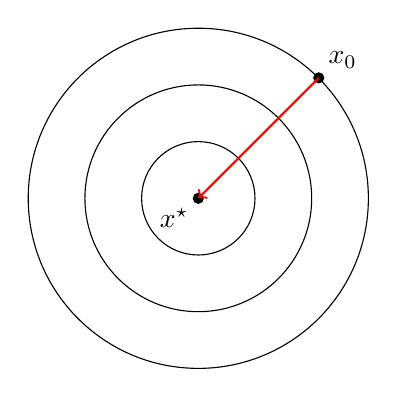
\begin{tikzpicture}[scale=0.9]
            \draw (0,0) circle (0.8cm);
            \draw (0,0) circle (1.6cm);
            \draw (0,0) circle (2.4cm);
            \filldraw (0,0) circle (2pt) node[below left] {$x^\star$};
            \coordinate (x0) at (1.7, 1.7);
            \filldraw (x0) circle (2pt) node[above right] {$x_0$};
            \draw[->, thick, red] (x0) -- (0,0);
        \end{tikzpicture}
        \caption{Valeurs propres égales ($Q=\lambda I$) : convergence directe en une itération.}
    \end{subfigure}
    
    \vspace{0.8cm}
    
    % Figure (b) - Valeurs propres différentes
    \begin{subfigure}[b]{\textwidth}
        \centering
        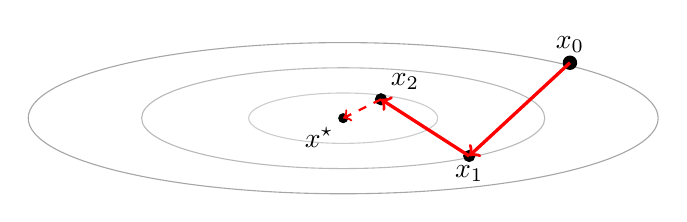
\begin{tikzpicture}[scale=0.8]
            % 3 ellipses horizontales allongées (mauvais conditionnement κ >> 1)
            \draw[gray!70] (0,0) ellipse (5cm and 1.2cm);
            \draw[gray!55] (0,0) ellipse (3.2cm and 0.8cm);
            \draw[gray!40] (0,0) ellipse (1.5cm and 0.4cm);
            
            % Point optimal au centre
            \filldraw (0,0) circle (2pt) node[below left] {$x^\star$};
            
            % Trajectoire avec zigzag simple et clair (3 flèches)
            % x0 sur l'ellipse (5, 1.2): (3.6, 0.88) vérifie environ x²/25 + y²/1.44 ≈ 1
            \coordinate (x0) at (3.6, 0.88);
            \coordinate (x1) at (2.0, -0.6);
            \coordinate (x2) at (0.6, 0.3);
            
            % Points avec labels bien positionnés
            \filldraw (x0) circle (3pt) node[above] {$x_0$};
            \filldraw (x1) circle (2.5pt) node[below] {$x_1$};
            \filldraw (x2) circle (2.5pt) node[above right] {$x_2$};
            
            % Flèches du zigzag
            \draw[->, very thick, red] (x0) -- (x1);
            \draw[->, very thick, red] (x1) -- (x2);
            \draw[->, thick, red, dashed] (x2) -- (0,0);
        \end{tikzpicture}
        \caption{Valeurs propres très différentes ($\kappa \gg 1$) : convergence lente en zigzag.}
    \end{subfigure}
    \caption{Effet du conditionnement de $Q$ sur la descente de gradient.}
\end{figure}

\textbf{Cas non linéaire:}
\begin{theoreme}
\label{thm:SD-nonlinear-rate}
Supposons que $f$ est deux fois différentiable et que les itérés générés par la
méthode de plus forte pente convergent vers un point $x^\star$ tel que la Hessienne
$\nabla^2 f(x^\star)$ soit définie positive. Soient
$\lambda_1 \le \cdots \le \lambda_m$ les valeurs propres de $\nabla^2 f(x^\star)$
et soit
\[
    \omega \in \left(\frac{\lambda_m - \lambda_1}{\lambda_m + \lambda_1}, 1\right).
\]
Alors, pour $k$ suffisamment grand,
\[
    f(x_{k+1}) - f(x^\star)
    \le \omega^2 \bigl( f(x_k) - f(x^\star) \bigr).
\]
\end{theoreme}

\begin{exemple}
Supposons que
\[
    f(x_0) = 1, \qquad f(x^\star) = 0,
\]
et que
\[
    \kappa\bigl(\nabla^2 f(x^\star)\bigr)
    = \|\nabla^2 f(x^\star)\|\;\bigl\|\bigl(\nabla^2 f(x^\star)\bigr)^{-1}\bigr\|
    = \frac{\lambda_m}{\lambda_1} = 800.
\]
Alors la constante de convergence linéaire est
\[
    \omega = \frac{800 - 1}{800 + 1}.
\]
Après $1000$ itérations,
\[
    f(x_{1001}) \approx \omega^{2000} f(x_0) \approx 0{,}082.
\]
\end{exemple}

\begin{definition}[Vitesse de convergence]
\label{def:convergence-rates}
Soit $(x_k)$ une suite convergeant vers $x^\star$.
\begin{itemize}
    \item On dit que $(x_k)$ converge \emph{Q-linéairement} vers $x^\star$ s’il existe
    $\omega \in (0,1)$ et $k_0$ tels que
    \[
        \frac{\|x_{k+1} - x^\star\|}{\|x_k - x^\star\|}
        \le \omega, \quad \forall k \ge k_0.
    \]
    \item La convergence est \emph{Q-superlinéaire} si
    \[
        \frac{\|x_{k+1} - x^\star\|}{\|x_k - x^\star\|}
        \xrightarrow[k\to\infty]{} 0.
    \]
    \item La convergence est \emph{Q-quadratique} s’il existe $M>0$ et $k_0$ tels que
    \[
        \frac{\|x_{k+1} - x^\star\|}{\|x_k - x^\star\|^2}
        \le M,\quad \forall k \ge k_0.
    \]
\end{itemize}
\end{definition}

%%%%%%%%%%%%%%%%%%%%%%%%%%%%%%%%%%%%%%%%%%%%%%%%%%%%%%%%%%%%
\subsection{Méthode de Newton : convergence quadratique}
\label{subsec:2.4.5}

\begin{theoreme}[Convergence quadratique de Newton]
\label{thm:Newton-quadratic}
Supposons que $f$ est de classe $\mathcal{C}^2$ et que $\nabla^2 f$ est Lipschitzienne
dans un voisinage d’une solution $x^\star$ vérifiant les conditions suffisantes
du second ordre (cf. \autoref{thm:second-order-sufficient}). Considérons la
méthode de Newton
\[
    x_{k+1} = x_k - \bigl(\nabla^2 f(x_k)\bigr)^{-1}\nabla f(x_k).
\]
Alors :
\begin{enumerate}
    \item si $x_0$ est assez proche de $x^\star$, la suite $(x_k)$ converge vers $x^\star$ ;
    \item la convergence est quadratique :
    \[
        \|x_{k+1} - x^\star\|
        \le C \|x_k - x^\star\|^2
    \]
    pour une constante $C>0$ et $k$ assez grand ;
    \item les normes de gradient satisfont également une convergence quadratique :
    \[
        \|\nabla f(x_{k+1})\|
        \le C' \|\nabla f(x_k)\|^2.
    \]
\end{enumerate}
\end{theoreme}

\begin{figure}[H]
\centering

\includegraphics[width=0.7\textwidth]{2.png}
\caption{Itérations de la méthode de Newton sur les courbes de niveau de la fonction de Rosenbrock.}
\label{fig:newton-rosenbrock}
\end{figure}

\begin{figureexplanation}
\textbf{Points clés à observer :}
\begin{itemize}
    \item \textbf{Trajectoire directe :} Contrairement à la descente de gradient (Figure~\ref{fig:steepest-descent-rosenbrock}), Newton atteint le minimum en très peu d'itérations.
    \item \textbf{Utilisation de la Hessienne :} L'information de courbure permet de « corriger » la direction du gradient pour suivre le fond de la vallée.
    \item \textbf{Convergence quadratique :} Proche du minimum, chaque itération double le nombre de chiffres significatifs corrects (théorème~\ref{thm:Newton-quadratic}).
    \item \textbf{Coût :} Chaque itération nécessite le calcul et l'inversion de la Hessienne, ce qui peut être prohibitif en grande dimension.
\end{itemize}
\end{figureexplanation}

%%%%%%%%%%%%%%%%%%%%%%%%%%%%%%%%%%%%%%%%%%%%%%%%%%%%%%%%%%%%
\subsection{Modification de la Hessienne pour Newton}
\label{subsec:2.4.6}

L’efficacité de la méthode de Newton repose sur la positivi\-té de la Hessienne.
Loin de la solution, il peut arriver que $\nabla^2 f_k$ ne soit pas définie positive,
de sorte que la direction
\[
    \eta_k^N = -(\nabla^2 f_k)^{-1}\nabla f_k
\]
ne soit pas une direction de descente.

On introduit alors une matrice $B_k$ qui joue le rôle de Hessienne modifiée,
et on résout
\[
    B_k \eta_k = -\nabla f_k.
\]

\begin{algorithm}[H]
\caption{Newton avec recherche linéaire et Hessienne modifiée}
\label{alg:newton-modified}
\KwInput{an initial point $x_0$}
\For{$k = 0, 1, \ldots$}{
    Factorize the matrix $B_k = \nabla^2 f(x_k) + E_k$, where $E_k = 0$ if $\nabla^2 f(x_k)$ is sufficiently positive definite. Otherwise, $E_k$ is chosen to ensure that $B_k$ is sufficiently positive definite\;
    Solve $B_k p_k = -\nabla f(x_k)$\;
    Set $x_{k+1} \leftarrow x_k + \alpha_k p_k$, where $\alpha_k$ satisfies the Wolfe, Goldstein, or Armijo backtracking conditions\;
}
\end{algorithm}

\begin{definition}[Propriété de factorisation modifiée bornée (BMFP)]
On dit que la suite $(B_k)$ satisfait la \emph{propriété de factorisation modifiée
bornée} (BMFP) s’il existe $C>0$ tel que
\[
    \kappa(B_k)
    = \|B_k\|\cdot\|B_k^{-1}\| \le C,
    \quad \forall k.
\]
\end{definition}

\begin{theoreme}[Moré--Sorensen]
\label{thm:More-Sorensen}
Supposons que $f$ est de classe $\mathcal{C}^2$ sur un ouvert $D\subset\mathbb{R}^n$.
Supposons que l’ensemble de niveau
\[
    \{ x \in \mathbb{R}^n \;|\; f(x) \le f(x_0)\}
\]
est compact. Si la suite $(B_k)$ utilisée dans l’algorithme de Newton modifié
satisfait la propriété BMFP, alors
\[
    \|\nabla f_k\| \xrightarrow[k\to\infty]{} 0.
\]
\end{theoreme}

\paragraph{Exemples de constructions de $B_k$.}

\begin{itemize}
    \item \textbf{Décomposition spectrale.} On peut diagonaliser $\nabla^2 f_k$,
    remplacer les valeurs propres non positives par une petite constante $\delta>0$
    (ou éventuellement renverser le signe des valeurs propres négatives), puis
    reconstruire la matrice.
    \item \textbf{Ajout d’un multiple de l’identité.} On cherche $\tau>0$ tel que
    $\nabla^2 f_k + \tau I$ soit définie positive.
\end{itemize}

\begin{algorithm}[H]
\caption{Cholesky avec ajout d'un multiple de l'identité}
\label{alg:Cholesky-identity}
Choose $\beta > 0$\;
\If{$\min_i(a_{i,i}) > 0$}{
    Set $\tau_0 \leftarrow 0$\;
}
\Else{
    $\tau_0 \leftarrow -\min_i(a_{i,i}) + \beta$\;
}
\For{$k = 0, 1, \ldots$}{
    Attempt to apply the Cholesky algorithm to obtain $LL' = A + \tau_k I$\;
    \If{the factorization is completed successfully}{
        \Stop \And \Return $L$\;
    }
    \Else{
        $\tau_{k+1} \leftarrow \max(2\tau_k, \beta)$\;
    }
}
\end{algorithm}

\paragraph{Factorisation de Cholesky modifiée.}

Toute matrice symétrique définie positive $A$ peut s’écrire $A = LDL^\top$ où
$D$ est diagonale et $L$ est triangulaire inférieure à diagonale unité.
On peut modifier l’algorithme de Cholesky pour assurer que les éléments de $D$
restent strictement positifs, ce qui fournit une méthode stable de construction
de matrices $B_k$ définies positives. Voir par exemple \cite{gill2019practical}
ou \cite{more1982newton} pour plus de détails.

%%%%%%%%%%%%%%%%%%%%%%%%%%%%%%%%%%%%%%%%%%%%%%%%%%%%%%%%%%%%
\section{Exercices d'entraînement (Nocedal \& Wright)}
\label{sec:2.exercises}

\subsection*{Partie 1 : Questions de cours (Type Examen)}
\bigskip
\begin{exercice}[Questions de compréhension]
\begin{enumerate}
    \item \textbf{Recherche linéaire :} Décrire le principe de la recherche linéaire ("Line Search"). Expliquer graphiquement la condition d'Armijo et la condition de courbure (Wolfe).
    \item \textbf{Newton vs Gradient :} Pourquoi préférerait-on la méthode de Newton à la méthode de plus forte pente ? Quel est le coût associé ?
    \item \textbf{Hessienne mal conditionnée :} Que faire si l'on souhaite implémenter la méthode de Newton mais que la Hessienne est très grande ou singulière ? (Discussion sur Newton Modifié, Quasi-Newton, ou Trust Region).
    \item \textbf{Taux de convergence :} Définir les taux de convergence linéaire, superlinéaire et quadratique. Donner un exemple de méthode pour chaque taux.
    \item \textbf{Direction de descente :} Montrer mathématiquement que si $B_k$ est définie positive, la direction $-B_k^{-1} \nabla f_k$ est toujours une direction de descente.
    \item \textbf{Scaling :} Expliquer comment le mauvais scaling des variables affecte la méthode de plus forte pente (Zig-zag).
\end{enumerate}
\end{exercice}

\begin{correction}
\begin{enumerate}
    \item \textbf{Line Search :} On cherche un pas $\alpha_k > 0$ le long d'une direction de descente $p_k$. Armijo assure une décroissance suffisante (droite $f(x_k) + c_1 \alpha \nabla f_k^T p_k$). Courbure assure qu'on ne fait pas de trop petits pas (pente augmente). \textit{(Faire un dessin avec une courbe convexe et les droites sécantes).}
    \item \textbf{Newton :} Convergence quadratique (très rapide) près de la solution vs convergence linéaire pour Gradient. Coût : Calcul et inversion (ou factorisation) de la Hessienne $O(n^3)$.
    \item \textbf{Large/Singular Hessian :}
    \begin{itemize}
        \item \textit{Newton Modifié :} Ajouter $\tau I$ (Cholesky modifiée) pour la rendre définie positive.
        \item \textit{Quasi-Newton (BFGS) :} Approximer $B_k$ itérativement (seulement gradients nécessaires, $O(n^2)$).
        \item \textit{Trust Region :} Limiter le pas à une zone de confiance si le modèle quadratique n'est pas bon.
        \item \textit{Newton-CG :} Résoudre le système linéaire par Gradient Conjugué tronqué (pas besoin de stocker la Hessienne explicite, juste produits matrice-vecteur).
    \end{itemize}
    \item \textbf{Définitions :} Voir Annexe A.
    \item \textbf{Descente :} $p_k^T \nabla f_k = - (\nabla f_k)^T B_k^{-1} \nabla f_k$. Posons $v = \nabla f_k$. On a $- v^T B_k^{-1} v$. Si $B_k \succ 0$, alors $B_k^{-1} \succ 0$, donc $v^T B_k^{-1} v > 0$ pour $v \ne 0$. Donc produit scalaire $< 0$, c'est une descente.
\end{enumerate}
\end{correction}
\bigskip

\subsection*{Partie 2 : Exercices d'application}

\bigskip
\begin{exercice}[Fonction de Rosenbrock]
Soit $f(x) = 100(x_2 - x_1^2)^2 + (1 - x_1)^2$.
\begin{enumerate}
    \item Calculer le gradient $\nabla f(x)$ et la Hessienne $\nabla^2 f(x)$.
    \item Trouver les points critiques.
    \item Vérifier les conditions suffisantes du second ordre (SOSC) pour confirmer la nature de ces points.
\end{enumerate}
\end{exercice}

\begin{correction}
\textbf{1. Calculs :}
$$ \nabla f(x) = \begin{pmatrix} -400x_1(x_2 - x_1^2) - 2(1-x_1) \\ 200(x_2 - x_1^2) \end{pmatrix} $$
$$ \nabla^2 f(x) = \begin{pmatrix} -400x_2 + 1200x_1^2 + 2 & -400x_1 \\ -400x_1 & 200 \end{pmatrix} $$

\textbf{2. Points Critiques (FOC) :}
$\nabla f(x) = 0$.
(ii) $200(x_2 - x_1^2) = 0 \implies x_2 = x_1^2$.
(i) $-400x_1(0) - 2(1-x_1) = 0 \implies x_1 = 1$.
Unique point stationnaire : $x^* = (1, 1)^T$.

\textbf{3. Conditions du Second Ordre (SOSC) :}
Évaluons la Hessienne en $x^*=(1,1)$.
$$ H = \nabla^2 f(1,1) = \begin{pmatrix} -400(1) + 1200(1) + 2 & -400 \\ -400 & 200 \end{pmatrix} = \begin{pmatrix} 802 & -400 \\ -400 & 200 \end{pmatrix} $$
Pour vérifier qu'elle est définie positive :
- Mineurs principaux : $M_1 = 802 > 0$.
- Déterminant : $\det(H) = 802(200) - (-400)^2 = 160400 - 160000 = 400 > 0$.
Les mineurs principaux dominants sont strictement positifs, donc $H \succ 0$.
\end{correction}
\bigskip
\bigskip
\begin{checkpoint}
\begin{itemize}
    \item \textbf{Optimalité :} Quelle est la condition nécessaire du premier ordre ($\nabla f = 0$) ? Et suffisante du second ordre ($\nabla^2 f \succ 0$) ?
    \item \textbf{Taylor :} Savez-vous écrire le développement de Taylor d'ordre 2 pour une fonction multivariée ?
    \item \textbf{Méthodes :} Quelle est la différence fondamentale entre la méthode de plus forte pente (Gradient Descent) et la méthode de Newton (utilisation de la courbure/Hessienne) ?
    \item \textbf{Convergence :} Qu'est-ce qu'une convergence quadratique ? Laquelle des deux méthodes ci-dessus la possède ?
\end{itemize}
\end{checkpoint}


\bigskip
\begin{exercice}[Contre-exemple Conditions de Wolfe]
Montrer que si $0 < c_2 < c_1 < 1$, il est possible qu'aucun pas $\alpha$ ne satisfasse les conditions de Wolfe.
\end{exercice}

\begin{correction}
La condition de courbure (Wolfe 2) demande $\nabla f(x_k + \alpha p_k)^T p_k \ge c_2 \nabla f_k^T p_k$.
Comme $\nabla f_k^T p_k < 0$ (direction de descente) et $c_2 < c_1$, la pente demandée est "moins négative" (plus plate) que celle permise par la condition d'Armijo stricte si la fonction est convexe/quadratique.
Si on a une fonction convexe quadratique, la pente croit de manière monotone.
La condition d'Armijo s'écrit $\phi(\alpha) \le \phi(0) + c_1 \alpha \phi'(0)$.
Si $c_2 < c_1$, l'intervalle admissible pour la courbure peut être disjoint de l'intervalle admissible pour Armijo, spécifiquement si la fonction remonte "trop vite" ou si les paramètres sont mal choisis par rapport à la courbure réelle.
(Voir Nocedal \& Wright Ex 3.2 pour les détails géométriques).
\end{correction}
\bigskip

\bigskip
\begin{exercice}[Méthode de plus forte pente sur une quadratique]
Considérer la méthode de plus forte pente avec recherche linéaire exacte appliquée à la fonction quadratique convexe $f(x) = \frac{1}{2}x^T Q x - b^T x$. 
Montrer que si le point initial est tel que $x_0 - x^*$ est parallèle à un vecteur propre de $Q$, alors la méthode trouve la solution en une seule étape.
\end{exercice}

\begin{correction}
Soit $x_0 - x^* = v$ où $Qv = \lambda v$.
Le gradient est $\nabla f(x) = Qx - b = Q(x - x^*) + (Qx^* - b) = Q(x-x^*)$.
Donc $\nabla f(x_0) = Q(x_0 - x^*) = \lambda (x_0 - x^*)$.
La direction de plus forte pente est $p_0 = -\nabla f(x_0) = -\lambda (x_0 - x^*)$.
C'est donc exactement la direction vers la solution $x^*$.
Une recherche linéaire exacte trouvera le minimum le long de cette ligne, qui est précisément $x^*$.
\end{correction}
\bigskip

\bigskip
\begin{exercice}[Taux de convergence - à discuter]
(Voir Annexe A.2 du livre pour les définitions exactes). 
\begin{enumerate}
    \item Montrer que la suite $x_k = 1/k$ n'est pas Q-linéairement convergente, bien qu'elle converge vers zéro. (Convergence sublinéaire).
    \item Montrer que la suite $x_k = 1 + (0.5)^{2^k}$ converge Q-quadratiquement vers 1.
    \item La suite $x_k = 1/k!$ converge-t-elle Q-superlinéairement ? Q-quadratiquement ?
\end{enumerate}
\end{exercice}

\begin{correction}
\begin{enumerate}
    \item Pour $x_k = 1/k$, le ratio $\frac{|x_{k+1}-0|}{|x_k-0|} = \frac{1/(k+1)}{1/k} = \frac{k}{k+1} \to 1$. Pour une convergence Q-linéaire, ce ratio doit être majoré par une constante $r < 1$. Ici ce n'est pas le cas.
    \item Erreur $e_k = (0.5)^{2^k}$.
    $e_{k+1} = (0.5)^{2^{k+1}} = (0.5)^{2 \cdot 2^k} = ((0.5)^{2^k})^2 = e_k^2$.
    Donc $\frac{e_{k+1}}{e_k^2} = 1$. C'est une convergence Q-quadratique.
    \item $x_k = 1/k!$. $e_k = 1/k!$.
    Ratio : $\frac{e_{k+1}}{e_k} = \frac{1}{(k+1)!} \cdot k! = \frac{1}{k+1} \to 0$. C'est donc Q-superlinéaire.
    Pour quadratique : $\frac{e_{k+1}}{e_k^2} = \frac{1}{(k+1)!} \cdot (k!)^2 = \frac{(k!)^2}{k!(k+1)} = \frac{k!}{k+1} \to \infty$.
    Donc ça converge moins vite que quadratiquement.
\end{enumerate}
\end{correction}
\bigskip
